\documentclass{article}



\usepackage{arxiv}

\usepackage[utf8]{inputenc} % allow utf-8 input
\usepackage[T1]{fontenc}    % use 8-bit T1 fonts
\usepackage{hyperref}       % hyperlinks
\usepackage{url}            % simple URL typesetting
\usepackage{booktabs}       % professional-quality tables
\usepackage{amsfonts}       % blackboard math symbols
\usepackage{nicefrac}       % compact symbols for 1/2, etc.
\usepackage{microtype}      % microtypography
\usepackage{lipsum}		% Can be removed after putting your text content
\usepackage{graphicx}
\usepackage{natbib}
\usepackage{doi}
\usepackage{listings,xcolor}
\lstdefinestyle{lua}{
  language=[5.3]Lua,
  basicstyle=\ttfamily,
  keywordstyle=\color{magenta},
  stringstyle=\color{blue},
  commentstyle=\color{black!50}
}


\title{Multidarkroom}

%\date{September 9, 1985}	% Here you can change the date presented in the paper title
%\date{} 					% Or removing it

\author{
    Denis Roio \\
	Dyne.org foundation \\
	Amsterdam, 1013AK \\
	\texttt{J@Dyne.org} \\
    \And
	Alberto Ibrisevic \\
	Laboratory of Cryptography\\
	Trento University (stage)\\
	\texttt{bettowski@dyne.org} \\
    \And
    Andrea D'Intino \\
    Dyne.org foundation \\
    Amsterdam, 1013AK \\
    \texttt{Andrea@Dyne.org} \\
}

% Uncomment to remove the date
%\date{}

% Uncomment to override  the `A preprint' in the header
\renewcommand{\headeright}{Dyne.org}
\renewcommand{\undertitle}{Zero Knowledge Multi Party Signatures with
  Application to Distributed Ledgers}
\renewcommand{\shorttitle}{\textit{Multidarkroom}}

%%% Add PDF metadata to help others organize their library
%%% Once the PDF is generated, you can check the metadata with
%%% $ pdfinfo template.pdf

\hypersetup{
pdftitle={Multidarkroom - Zero-knowledge proof secured BLS multi-signatures},
pdfsubject={cs.CR},
pdfauthor={Denis Roio, Alberto Ibrisevic, Andrea D'Intino},
pdfkeywords={Cryptography, signatures, zero-knowledge, multi-party, BLS, Coconut},
}

\begin{document}
\maketitle

\begin{abstract}
  Multidarkroom is a novel signature scheme supporting unlinkable
  signatures by multiple parties authenticated by means of a
  zero-knowledge credential scheme. Multidarkroom integrates with
  blockchains to ensure condidentiality, authenticity and availability
  even when credential issuing authorities are offline. We implement
  and evaluate a Multidarkroom smart contract for Zenroom and present
  an application related to multiple anonymous signatures by
  authenticated parties. Multidarkroom uses short and computationally
  efficient signatures and credentials whose verification takes the
  longest time to compute.
\end{abstract}


% keywords can be removed
% \keywords{First keyword \and Second keyword \and More}


\section{Introduction}

Multi-party computation [] applied to the signing process [] allows
the issuance of signatures without requiring any of the participating
parties to disclose secret signing keys to each other, nor requires
the presence of a trusted third-party to receive them and compose the
signatures. However, established schemes have shortcomings. Some do
not provide the necessary efficiency, re-randomization, or blind
issuance properties necessary to implement the privacy preserving
features necessary for the application to trustless distributed
systems. Other schemes are prone to rogue-key attacks \citep{ietf-bls}
in the absence of authentication methods to grant that signatures are
produced by legitimate key holders.

The lack of efficient and privacy-preserving signature schemes impacts
distributed ledger platforms that support 'smart contracts' as well
distributed computing architectures where trust is not shared among
participants, but granted by one or more authorities through
credential issuance for the generation of non-interactive and
unlinkable proofs.

Multidarkroom uses short and computationally efficient signatures
composed of exactly two group elements that are linked to each
other. The size of the signature remains constant regardless of the
number of parties that are signing, while the credential size grows
linearly. Furthermure, after a one-time setup phase where the users
collect and aggregate a threshold number of verification keys from the
autorities, the attribute showing and verification O(1) in terms of
both cryptographic computations and communication of cryptographic
material, irrespective of the number of authorities.

Our evaluationof the Multiparty primities shows very promising
results. Verifiction takes about 10ms,  while signing a document is
about 3 times faster. 

\subsection{Contributions}

This paper makes three key contributions:

\begin{itemize}

\item We describe the credential scheme underlying Multidarkroom,
  including how key generation, issuance, aggregation and verification
  of credentials operate (Section II). The scheme is an application of
  the Coconut credential scheme \citep{coconut-2018} that is general
  purpose and can be scaled to a fully distributed threshold issuance
  that is re-randomizable.

\item We describe the signature scheme underlying Multidarkroom,
  including how key generation, signing and verification operate (
  \ref{sec:signature}). The scheme is an application of the BLS
  signature scheme [] fitted with features to grant the unlinkability
  of signatures and to secure it against rogue-key attacks.

\item We use Multidarkroom to implement a Zencode scenario to be
  executed on and off-chain by the Zenroom VM, complete with functions
  for public credential issuance, signature session creation and
  multi-party non-interactive signing (Section III). We evaluate the
  performance and cost of this implementation on on-site and on-line
  platforms leveraging end-to-end encryption (Section VI).

\end{itemize}

% I. Signature scheme (BLS)
\section{Signature}
\label{sec:signature}

\lipsum[1]

\subsection{Vulnerability}
\lipsum[2]

% \begin{equation}
% 	\xi _{ij}(t)=P(x_{t}=i,x_{t+1}=j|y,v,w;\theta)= {\frac {\alpha _{i}(t)a^{w_t}_{ij}\beta _{j}(t+1)b^{v_{t+1}}_{j}(y_{t+1})}{\sum _{i=1}^{N} \sum _{j=1}^{N} \alpha _{i}(t)a^{w_t}_{ij}\beta _{j}(t+1)b^{v_{t+1}}_{j}(y_{t+1})}}
% \end{equation}

\section{Credential}
\label{sec:credential}

\lipsum[3]

\section{Implementation}

In this section we illustrate our implementation of Multidarkroom
keygen, sign and verify operations outlining for each:

\begin{enumerate}
  \item the communication sequence diagram
  \item the Zenroom code (Lua dialect)
  \item the Zencode statements
\end{enumerate}


\subsection{Keygen}

\begin{figure}
  \caption{Keygen process sequence diagram}
  \centering
  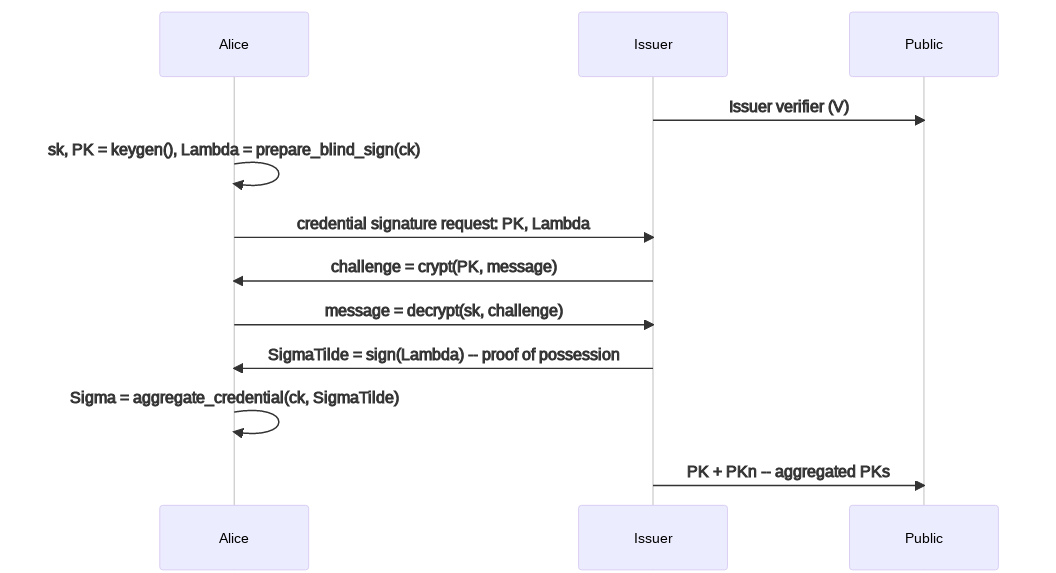
\includegraphics[width=0.8\textwidth]{keygen-seq}
\end{figure}

\subsection{Sign}

\begin{figure}
  \caption{Signing process sequence diagram}
  \centering
  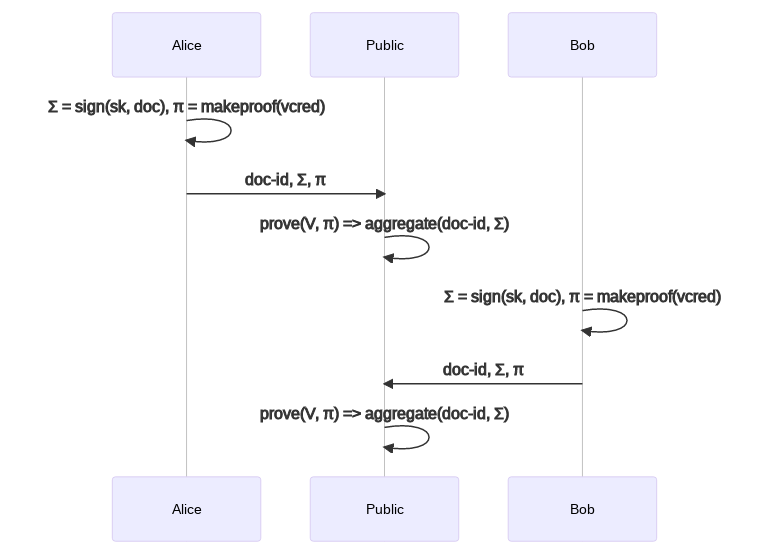
\includegraphics[width=0.8\textwidth]{sign-seq}
\end{figure}

\subsection{Verify}

\begin{figure}
  \caption{Verification process sequence diagram}
  \centering
  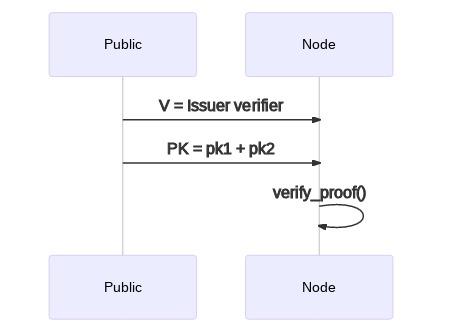
\includegraphics[width=0.8\textwidth]{verify-seq}
\end{figure}



\begin{lstlisting}[style=lua]

---------
-- SETUP
---------

G1 = ECP.generator()
G2 = ECP2.generator()

-- credentials
ZK = require_once('crypto_abc')
issuer = ZK.issuer_keygen()

-- keygen
sk1 = INT.random() -- signing key
ck1 = INT.random() -- credential key
PK1 = G2 * sk1     -- signature verifier

sk2 = INT.random()
ck2 = INT.random()
PK2 = G2 * sk2

-- issuer sign ZK credentials
Lambda1 = ZK.prepare_blind_sign(ck1*G1, ck1) -- credential request:       p -> i
SigmaTilde1 = ZK.blind_sign(issuer.sign, Lambda1)    -- issuer signs credential:  i -> p
Sigma1 = ZK.aggregate_creds(ck1, {SigmaTilde1})  -- credential sigma          p -> store

Lambda2 = ZK.prepare_blind_sign(ck2*G1, ck2)
SigmaTilde2 = ZK.blind_sign(issuer.sign, Lambda2)
Sigma2 = ZK.aggregate_creds(ck2, {SigmaTilde2})

-- sign

UID = ECP.hashtopoint(msg) -- the message's hash is the unique identifier

--------------
-- SETUP done
--------------

print "--------------------------"
print "first base signing session"
r = INT.random()
R = UID * r      -- session

-- add public keys to public session key
PM = (G2 * r) + PK1 + PK2

-- Session opener broadcasts:
-- 1. R   - base G1 point for signature session
-- 2. PM  - base G2 point for public multi-signature key
-- 3. msg - the message to be signed

-- proofs of valid signature
-- uses public session key as UID
Proof1,z1 = ZK.prove_cred_uid(issuer.verify, Sigma1, ck1, UID)
Proof2,z2 = ZK.prove_cred_uid(issuer.verify, Sigma2, ck2, UID)
-- each signer signs
S1 = UID * sk1
S2 = UID * sk2

-- generate the signature
-- each signer will communicate: UID * sk
SM = R + S1 + S2


-- print signature contents to screen
I.print({pub = PM, -- session public keys
		 sign = SM,
		 uid = UID,
		 proofhash1 = sha256( ZEN.serialize( Proof1 ) ),
		 proofhash2 = sha256( ZEN.serialize( Proof2 ) ),
		 zeta1 = z1,
		 zeta2 = z2,
		 issuer = issuer.verify
})

-- verify
assert( ZK.verify_cred_uid(issuer.verify, Proof1, z1, UID),
		"first proof verification fails")
assert( ZK.verify_cred_uid(issuer.verify, Proof2, z2, UID),
		"second proof verification fails")
assert( ECP2.miller(PM, UID)
		   == ECP2.miller(G2, SM),
        "Signature doesn't validates")

\end{lstlisting}

\section{Evaluation}

\lipsum[5]

\section{Bibliography}

\bibliographystyle{unsrtnat}

\bibliography{references}



% \subsection{}
% Citations use \verb+natbib+. The documentation may be found at
% \begin{center}
% 	\url{http://mirrors.ctan.org/macros/latex/contrib/natbib/natnotes.pdf}
% \end{center}

% Here is an example usage of the two main commands (\verb+citet+ and \verb+citep+): Some people thought a thing \citep{kour2014real, hadash2018estimate} but other people thought something else \citep{kour2014fast}. Many people have speculated that if we knew exactly why \citet{kour2014fast} thought this\dots

% \subsection{Figures}
% \lipsum[10]
% See Figure \ref{fig:fig1}. Here is how you add footnotes. \footnote{Sample of the first footnote.}
% \lipsum[11]

% \begin{figure}
% 	\centering
% 	\fbox{\rule[-.5cm]{4cm}{4cm} \rule[-.5cm]{4cm}{0cm}}
% 	\caption{Sample figure caption.}
% 	\label{fig:fig1}
% \end{figure}

% \subsection{Tables}
% See awesome Table~\ref{tab:table}.

% The documentation for \verb+booktabs+ (`Publication quality tables in LaTeX') is available from:
% \begin{center}
% 	\url{https://www.ctan.org/pkg/booktabs}
% \end{center}


% \begin{table}
% 	\caption{Sample table title}
% 	\centering
% 	\begin{tabular}{lll}
% 		\toprule
% 		\multicolumn{2}{c}{Part}                   \\
% 		\cmidrule(r){1-2}
% 		Name     & Description     & Size ($\mu$m) \\
% 		\midrule
% 		Dendrite & Input terminal  & $\sim$100     \\
% 		Axon     & Output terminal & $\sim$10      \\
% 		Soma     & Cell body       & up to $10^6$  \\
% 		\bottomrule
% 	\end{tabular}
% 	\label{tab:table}
% \end{table}



\end{document}
